\documentclass{ximera}

%\usepackage{todonotes}

\newcommand{\todo}{}

\usepackage{esint} % for \oiint
\ifxake%%https://math.meta.stackexchange.com/questions/9973/how-do-you-render-a-closed-surface-double-integral
\renewcommand{\oiint}{{\large\bigcirc}\kern-1.56em\iint}
\fi


\graphicspath{
  {./}
  {ximeraTutorial/}
  {basicPhilosophy/}
  {functionsOfSeveralVariables/}
  {normalVectors/}
  {lagrangeMultipliers/}
  {vectorFields/}
  {greensTheorem/}
  {shapeOfThingsToCome/}
  {dotProducts/}
  {partialDerivativesAndTheGradientVector/}
  {../productAndQuotientRules/exercises/}
  {../normalVectors/exercisesParametricPlots/}
  {../continuityOfFunctionsOfSeveralVariables/exercises/}
  {../partialDerivativesAndTheGradientVector/exercises/}
  {../directionalDerivativeAndChainRule/exercises/}
  {../commonCoordinates/exercisesCylindricalCoordinates/}
  {../commonCoordinates/exercisesSphericalCoordinates/}
  {../greensTheorem/exercisesCurlAndLineIntegrals/}
  {../greensTheorem/exercisesDivergenceAndLineIntegrals/}
  {../shapeOfThingsToCome/exercisesDivergenceTheorem/}
  {../greensTheorem/}
  {../shapeOfThingsToCome/}
  {../separableDifferentialEquations/exercises/}
  {vectorFields/}
}

\newcommand{\mooculus}{\textsf{\textbf{MOOC}\textnormal{\textsf{ULUS}}}}

\usepackage{tkz-euclide}
\usepackage{tikz}
\usepackage{tikz-cd}
\usetikzlibrary{arrows}
\tikzset{>=stealth,commutative diagrams/.cd,
  arrow style=tikz,diagrams={>=stealth}} %% cool arrow head
\tikzset{shorten <>/.style={ shorten >=#1, shorten <=#1 } } %% allows shorter vectors

\usetikzlibrary{backgrounds} %% for boxes around graphs
\usetikzlibrary{shapes,positioning}  %% Clouds and stars
\usetikzlibrary{matrix} %% for matrix
\usepgfplotslibrary{polar} %% for polar plots
\usepgfplotslibrary{fillbetween} %% to shade area between curves in TikZ
%\usetkzobj{all}
\usepackage[makeroom]{cancel} %% for strike outs
%\usepackage{mathtools} %% for pretty underbrace % Breaks Ximera
%\usepackage{multicol}
\usepackage{pgffor} %% required for integral for loops



%% http://tex.stackexchange.com/questions/66490/drawing-a-tikz-arc-specifying-the-center
%% Draws beach ball
\tikzset{pics/carc/.style args={#1:#2:#3}{code={\draw[pic actions] (#1:#3) arc(#1:#2:#3);}}}



\usepackage{array}
\setlength{\extrarowheight}{+.1cm}
\newdimen\digitwidth
\settowidth\digitwidth{9}
\def\divrule#1#2{
\noalign{\moveright#1\digitwidth
\vbox{\hrule width#2\digitwidth}}}




% \newcommand{\RR}{\mathbb R}
% \newcommand{\R}{\mathbb R}
% \newcommand{\N}{\mathbb N}
% \newcommand{\Z}{\mathbb Z}

\newcommand{\sagemath}{\textsf{SageMath}}


%\renewcommand{\d}{\,d\!}
%\renewcommand{\d}{\mathop{}\!d}
%\newcommand{\dd}[2][]{\frac{\d #1}{\d #2}}
%\newcommand{\pp}[2][]{\frac{\partial #1}{\partial #2}}
% \renewcommand{\l}{\ell}
%\newcommand{\ddx}{\frac{d}{\d x}}

% \newcommand{\zeroOverZero}{\ensuremath{\boldsymbol{\tfrac{0}{0}}}}
%\newcommand{\inftyOverInfty}{\ensuremath{\boldsymbol{\tfrac{\infty}{\infty}}}}
%\newcommand{\zeroOverInfty}{\ensuremath{\boldsymbol{\tfrac{0}{\infty}}}}
%\newcommand{\zeroTimesInfty}{\ensuremath{\small\boldsymbol{0\cdot \infty}}}
%\newcommand{\inftyMinusInfty}{\ensuremath{\small\boldsymbol{\infty - \infty}}}
%\newcommand{\oneToInfty}{\ensuremath{\boldsymbol{1^\infty}}}
%\newcommand{\zeroToZero}{\ensuremath{\boldsymbol{0^0}}}
%\newcommand{\inftyToZero}{\ensuremath{\boldsymbol{\infty^0}}}



% \newcommand{\numOverZero}{\ensuremath{\boldsymbol{\tfrac{\#}{0}}}}
% \newcommand{\dfn}{\textbf}
% \newcommand{\unit}{\,\mathrm}
% \newcommand{\unit}{\mathop{}\!\mathrm}
% \newcommand{\eval}[1]{\bigg[ #1 \bigg]}
% \newcommand{\seq}[1]{\left( #1 \right)}
% \renewcommand{\epsilon}{\varepsilon}
% \renewcommand{\phi}{\varphi}


% \renewcommand{\iff}{\Leftrightarrow}

% \DeclareMathOperator{\arccot}{arccot}
% \DeclareMathOperator{\arcsec}{arcsec}
% \DeclareMathOperator{\arccsc}{arccsc}
% \DeclareMathOperator{\si}{Si}
% \DeclareMathOperator{\scal}{scal}
% \DeclareMathOperator{\sign}{sign}


%% \newcommand{\tightoverset}[2]{% for arrow vec
%%   \mathop{#2}\limits^{\vbox to -.5ex{\kern-0.75ex\hbox{$#1$}\vss}}}
% \newcommand{\arrowvec}[1]{{\overset{\rightharpoonup}{#1}}}
% \renewcommand{\vec}[1]{\arrowvec{\mathbf{#1}}}
% \renewcommand{\vec}[1]{{\overset{\boldsymbol{\rightharpoonup}}{\mathbf{#1}}}}

% \newcommand{\point}[1]{\left(#1\right)} %this allows \vector{ to be changed to \vector{ with a quick find and replace
% \newcommand{\pt}[1]{\mathbf{#1}} %this allows \vec{ to be changed to \vec{ with a quick find and replace
% \newcommand{\Lim}[2]{\lim_{\point{#1} \to \point{#2}}} %Bart, I changed this to point since I want to use it.  It runs through both of the exercise and exerciseE files in limits section, which is why it was in each document to start with.

% \DeclareMathOperator{\proj}{\mathbf{proj}}
% \newcommand{\veci}{{\boldsymbol{\hat{\imath}}}}
% \newcommand{\vecj}{{\boldsymbol{\hat{\jmath}}}}
% \newcommand{\veck}{{\boldsymbol{\hat{k}}}}
% \newcommand{\vecl}{\vec{\boldsymbol{\l}}}
% \newcommand{\uvec}[1]{\mathbf{\hat{#1}}}
% \newcommand{\utan}{\mathbf{\hat{t}}}
% \newcommand{\unormal}{\mathbf{\hat{n}}}
% \newcommand{\ubinormal}{\mathbf{\hat{b}}}

% \newcommand{\dotp}{\bullet}
% \newcommand{\cross}{\boldsymbol\times}
% \newcommand{\grad}{\boldsymbol\nabla}
% \newcommand{\divergence}{\grad\dotp}
% \newcommand{\curl}{\grad\cross}
%\DeclareMathOperator{\divergence}{divergence}
%\DeclareMathOperator{\curl}[1]{\grad\cross #1}
% \newcommand{\lto}{\mathop{\longrightarrow\,}\limits}

% \renewcommand{\bar}{\overline}

\colorlet{textColor}{black}
\colorlet{background}{white}
\colorlet{penColor}{blue!50!black} % Color of a curve in a plot
\colorlet{penColor2}{red!50!black}% Color of a curve in a plot
\colorlet{penColor3}{red!50!blue} % Color of a curve in a plot
\colorlet{penColor4}{green!50!black} % Color of a curve in a plot
\colorlet{penColor5}{orange!80!black} % Color of a curve in a plot
\colorlet{penColor6}{yellow!70!black} % Color of a curve in a plot
\colorlet{fill1}{penColor!20} % Color of fill in a plot
\colorlet{fill2}{penColor2!20} % Color of fill in a plot
\colorlet{fillp}{fill1} % Color of positive area
\colorlet{filln}{penColor2!20} % Color of negative area
\colorlet{fill3}{penColor3!20} % Fill
\colorlet{fill4}{penColor4!20} % Fill
\colorlet{fill5}{penColor5!20} % Fill
\colorlet{gridColor}{gray!50} % Color of grid in a plot

\newcommand{\surfaceColor}{violet}
\newcommand{\surfaceColorTwo}{redyellow}
\newcommand{\sliceColor}{greenyellow}




\pgfmathdeclarefunction{gauss}{2}{% gives gaussian
  \pgfmathparse{1/(#2*sqrt(2*pi))*exp(-((x-#1)^2)/(2*#2^2))}%
}


%%%%%%%%%%%%%
%% Vectors
%%%%%%%%%%%%%

%% Simple horiz vectors
\renewcommand{\vector}[1]{\left\langle #1\right\rangle}


%% %% Complex Horiz Vectors with angle brackets
%% \makeatletter
%% \renewcommand{\vector}[2][ , ]{\left\langle%
%%   \def\nextitem{\def\nextitem{#1}}%
%%   \@for \el:=#2\do{\nextitem\el}\right\rangle%
%% }
%% \makeatother

%% %% Vertical Vectors
%% \def\vector#1{\begin{bmatrix}\vecListA#1,,\end{bmatrix}}
%% \def\vecListA#1,{\if,#1,\else #1\cr \expandafter \vecListA \fi}

%%%%%%%%%%%%%
%% End of vectors
%%%%%%%%%%%%%

%\newcommand{\fullwidth}{}
%\newcommand{\normalwidth}{}



%% makes a snazzy t-chart for evaluating functions
%\newenvironment{tchart}{\rowcolors{2}{}{background!90!textColor}\array}{\endarray}

%%This is to help with formatting on future title pages.
\newenvironment{sectionOutcomes}{}{}



%% Flowchart stuff
%\tikzstyle{startstop} = [rectangle, rounded corners, minimum width=3cm, minimum height=1cm,text centered, draw=black]
%\tikzstyle{question} = [rectangle, minimum width=3cm, minimum height=1cm, text centered, draw=black]
%\tikzstyle{decision} = [trapezium, trapezium left angle=70, trapezium right angle=110, minimum width=3cm, minimum height=1cm, text centered, draw=black]
%\tikzstyle{question} = [rectangle, rounded corners, minimum width=3cm, minimum height=1cm,text centered, draw=black]
%\tikzstyle{process} = [rectangle, minimum width=3cm, minimum height=1cm, text centered, draw=black]
%\tikzstyle{decision} = [trapezium, trapezium left angle=70, trapezium right angle=110, minimum width=3cm, minimum height=1cm, text centered, draw=black]


\title{Vectors}

\begin{document}

\begin{abstract}
algebraic geometry
\end{abstract}
\maketitle






Our real line is full, but quadratic functions have shown us that we still need some new numbers.  \\

To accomodate our need for new zeros, we are attempting to juggle two copies of the real numbers. Visually, we are organizing the two copies as two number lines drawn at right angles to each other.  This is reminding us of the Cartesian plane.  Therefore, we are using our ideas of the Cartesian plane to help us think about a new number system.  \\



In the Cartesian plane, the two axis give rise to a 2-dimensional plane full of points.  We are adopting the same idea for our new number system.  It will be full of 2-dimensional numbers.


We are in the process of inventing an arithmetic for our 2-dimensional numbers.  We begin by adopting the arrow explanations of addition and subtraction that we used on the traditional number line. The arrows are now 2-dimensional arrows called \textbf{vectors}, but they follow the same rules as before.

The next step is to invent some algebraic symbols for the vectors, so that we can think algebraically about the 2-dimensional numbers.


$\blacktriangleright$ We already use parentheses for describing points, dots, or locations on the plane: $(2, 3)$.


$\blacktriangleright$ We will use triangular brackets to describe vectors: $\langle 2, 3 \rangle$.  

Rather than a position, vectors describe numbers through length and direction - just like arrows on the traditional number line. 



\begin{notation}  \textbf{\textcolor{blue!55!black}{Vectors}} \\


When giving vectors a name, we often put an arrow over the name, $\vec{v}$, to let people know we are representing a vector. \\

Double vertical bars represent length: $|| \vec{v} ||$.

If $\vec{v} = \langle a, b \rangle$, then $|| \vec{v} || = || \langle a, b \rangle || = \sqrt{a^2 + b^2}$

\end{notation}


\textbf{Note:} Vector length is an application of the Pythagorean Theorem.  The legs of the right triangle are the vector components.  The arrow representing the vector is the hypotenuse of the right trangle.


\begin{example} Name and Length \\

Let $\vec{v} = \langle 2, 3 \rangle$. \\

Then, $|| \vec{v} || = || \langle 2, 3 \rangle || = \sqrt{2^2 + 3^2} = \sqrt{13}$

\end{example}







\begin{question} 


The length of  $\langle 3, 4 \rangle$ is $\answer{5}$.



\end{question}






\begin{question} 


The length of  $\langle -3, 4 \rangle$ is $\answer{5}$.



\end{question}



\begin{question} 


The length of  $\langle -2, 3 \rangle$ is $\answer{\sqrt{13}}$.



\end{question}




Vectors are the mental concept and we represent these visually with arrows. Many arrows may represent the same vector.  Their placement in the Cartesian plane will represent operations.


The numbers inside the parentheses for a point are called \textbf{\textcolor{purple!85!blue}{coordinates}}  

The numbers inside the triangular brackets for vectors are called \textbf{\textcolor{purple!85!blue}{components}}  



The geometry of the arrows has already suggested the algebraic procedures.


\begin{example}


$\langle 4, 6 \rangle + \langle 2, -10 \rangle$


\begin{image}
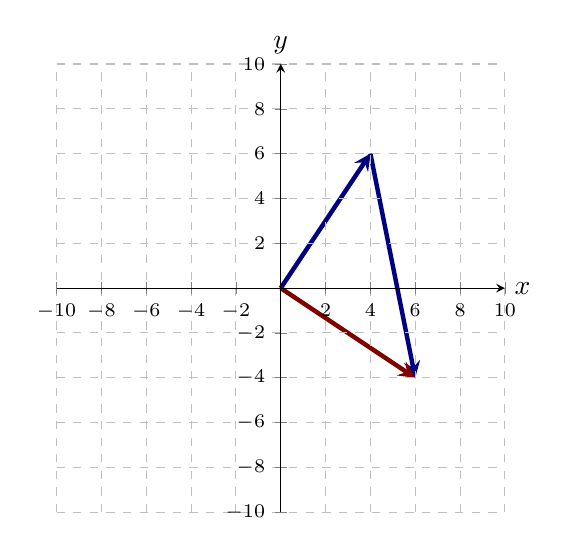
\begin{tikzpicture}
  \begin{axis}[
            domain=-10:10, ymax=10, xmax=10, ymin=-10, xmin=-10,
            axis lines =center, xlabel=$x$, ylabel=$y$, grid = major, grid style={dashed},
            unit vector ratio*=1 1 1,
            ytick={-10,-8,-6,-4,-2,2,4,6,8,10},
            xtick={-10,-8,-6,-4,-2,2,4,6,8,10},
            yticklabels={$-10$,$-8$,$-6$,$-4$,$-2$,$2$,$4$,$6$,$8$,$10$}, 
            xticklabels={$-10$,$-8$,$-6$,$-4$,$-2$,$2$,$4$,$6$,$8$,$10$},
            ticklabel style={font=\scriptsize},
            every axis y label/.style={at=(current axis.above origin),anchor=south},
            every axis x label/.style={at=(current axis.right of origin),anchor=west},
            axis on top
          ]


            \draw[penColor,ultra thick,->] (axis cs:0,0) -- (axis cs:4,6);
            \draw[penColor,ultra thick,->] (axis cs:4,6) -- (axis cs:6,-4);
            \draw[penColor2,ultra thick,->] (axis cs:0,0) -- (axis cs:6,-4);



  \end{axis}
\end{tikzpicture}
\end{image}


$\langle 4, 6 \rangle + \langle 2, 10 \rangle = \langle 4+2, 6+(-10) \rangle = \langle 6, -4 \rangle$


\end{example}





Algebraically, addition and subtraction of vectors will be carried out component-wise.



\begin{definition}  \textbf{\textcolor{green!50!black}{Vector Arithmetic}}  \\




\[     \langle A, B \rangle + \langle C, D \rangle = \langle A+C, B+D \rangle       \]


\[     \langle A, B \rangle - \langle C, D \rangle = \langle A-C, B-D \rangle       \]


\end{definition}







\begin{question} 


$\langle 3, 4 \rangle + \langle -2, 5 \rangle = \left\langle \answer{1}, \answer{9} \right\rangle$.



\end{question}








\subsection*{Scalars}

We also have several ideas about manipulating a single vector. \\



\begin{itemize}
\item We can think of add a vector to itself several times.
\item We can thnink of stretching or compressing a vector.
\item We can think of reversing a vector.
\end{itemize}



$\blacktriangleright$  Adding three copies of the same vector.

\begin{image}
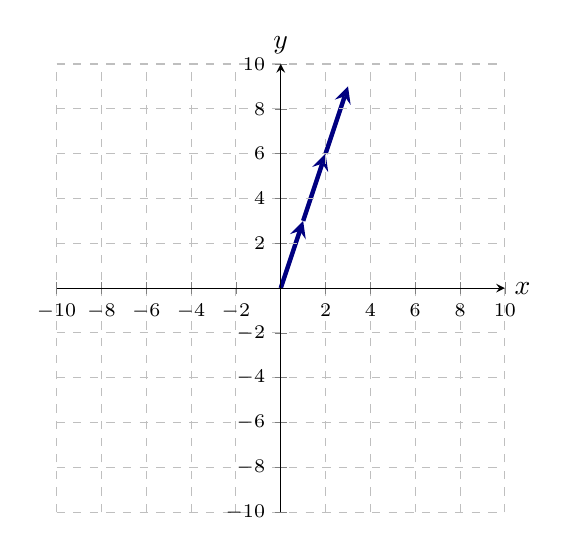
\begin{tikzpicture}
  \begin{axis}[
            domain=-10:10, ymax=10, xmax=10, ymin=-10, xmin=-10,
            axis lines =center, xlabel=$x$, ylabel=$y$, grid = major, grid style={dashed},
            unit vector ratio*=1 1 1,
            ytick={-10,-8,-6,-4,-2,2,4,6,8,10},
            xtick={-10,-8,-6,-4,-2,2,4,6,8,10},
            yticklabels={$-10$,$-8$,$-6$,$-4$,$-2$,$2$,$4$,$6$,$8$,$10$}, 
            xticklabels={$-10$,$-8$,$-6$,$-4$,$-2$,$2$,$4$,$6$,$8$,$10$},
            ticklabel style={font=\scriptsize},
            every axis y label/.style={at=(current axis.above origin),anchor=south},
            every axis x label/.style={at=(current axis.right of origin),anchor=west},
            axis on top
          ]


            \draw[penColor,ultra thick,->] (axis cs:0,0) -- (axis cs:1,3);
            \draw[penColor,ultra thick,->] (axis cs:1,3) -- (axis cs:2,6);
            \draw[penColor,ultra thick,->] (axis cs:2,6) -- (axis cs:3,9);



  \end{axis}
\end{tikzpicture}
\end{image}






$\blacktriangleright$  Compressing a vector to half its length.

\begin{image}
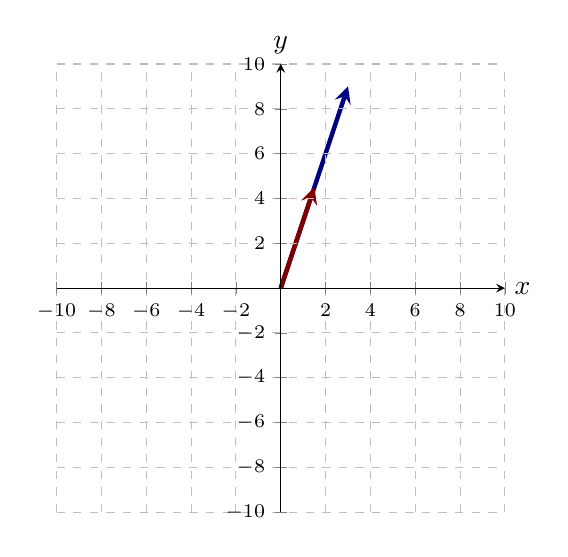
\begin{tikzpicture}
  \begin{axis}[
            domain=-10:10, ymax=10, xmax=10, ymin=-10, xmin=-10,
            axis lines =center, xlabel=$x$, ylabel=$y$, grid = major, grid style={dashed},
            unit vector ratio*=1 1 1,
            ytick={-10,-8,-6,-4,-2,2,4,6,8,10},
            xtick={-10,-8,-6,-4,-2,2,4,6,8,10},
            yticklabels={$-10$,$-8$,$-6$,$-4$,$-2$,$2$,$4$,$6$,$8$,$10$}, 
            xticklabels={$-10$,$-8$,$-6$,$-4$,$-2$,$2$,$4$,$6$,$8$,$10$},
            ticklabel style={font=\scriptsize},
            every axis y label/.style={at=(current axis.above origin),anchor=south},
            every axis x label/.style={at=(current axis.right of origin),anchor=west},
            axis on top
          ]


            \draw[penColor,ultra thick,->] (axis cs:0,0) -- (axis cs:3,9);
            \draw[penColor2,ultra thick,->] (axis cs:0,0) -- (axis cs:1.5,4.5);




  \end{axis}
\end{tikzpicture}
\end{image}










$\blacktriangleright$  Reversing the direction of a vector.

\begin{image}
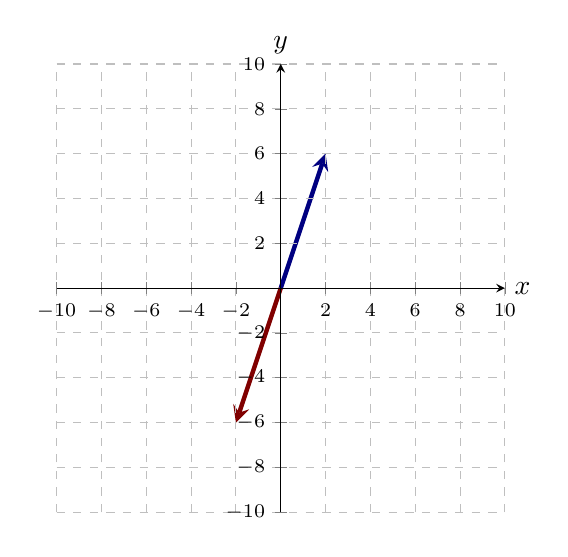
\begin{tikzpicture}
  \begin{axis}[
            domain=-10:10, ymax=10, xmax=10, ymin=-10, xmin=-10,
            axis lines =center, xlabel=$x$, ylabel=$y$, grid = major, grid style={dashed},
            unit vector ratio*=1 1 1,
            ytick={-10,-8,-6,-4,-2,2,4,6,8,10},
            xtick={-10,-8,-6,-4,-2,2,4,6,8,10},
            yticklabels={$-10$,$-8$,$-6$,$-4$,$-2$,$2$,$4$,$6$,$8$,$10$}, 
            xticklabels={$-10$,$-8$,$-6$,$-4$,$-2$,$2$,$4$,$6$,$8$,$10$},
            ticklabel style={font=\scriptsize},
            every axis y label/.style={at=(current axis.above origin),anchor=south},
            every axis x label/.style={at=(current axis.right of origin),anchor=west},
            axis on top
          ]


            \draw[penColor,ultra thick,->] (axis cs:0,0) -- (axis cs:2,6);
            \draw[penColor2,ultra thick,->] (axis cs:0,0) -- (axis cs:-2,-6);




  \end{axis}
\end{tikzpicture}
\end{image}



To describe these operations, we use \textbf{scalars}.


\begin{definition}  \textbf{\textcolor{green!50!black}{Scalars}}  \\

A \textbf{scalar} is the new name for our old real numbers. 

\end{definition}


Scalar multiplication is how we describe adding copies, stretching or compressing, or reversing the direction of vectors.


\begin{definition}  \textbf{\textcolor{green!50!black}{Scalar Multiplication}}  \\

\[    r \cdot \langle A, B \rangle  = \langle r \cdot A, r \cdot B \rangle   \text{ where }  r \in \mathbb{R}   \]

or, just

\[    r \, \langle A, B \rangle  = \langle r \, A, r \, B \rangle   \text{ where }  r \in \mathbb{R}   \]

\end{definition}









\begin{question} 


$5 \, \langle 3, -4 \rangle  = \left\langle \answer{15}, \answer{-20} \right\rangle$.



\end{question}









\begin{question} 


$-3 \, \langle -2, 7 \rangle  = \left\langle \answer{6}, \answer{-21} \right\rangle$.



\end{question}







Of course, scalars (our old real numbers) are also numbers in our new system.  They must also have a vector form. \\




\textbf{Real Numbers}



We haven't lost our 1-dimensional real numbers. Now, they are just embedded inside our new algebraic plane.  We can view the horizontal axis as the traditional real number line.

Each real number $r$ is now either represented by the point $(r,0)$ or by the horizontal vector, $\langle r, 0 \rangle$.  All of our operations are duplicated with these new visual tools along the horizontal axis.


\begin{itemize}
\item $1$ is now either $(1,0)$ or $\langle 1, 0 \rangle$.
\item $-1$ is now either $(-1,0)$ or $\langle -1, 0 \rangle$.
\item $0$ is now either $(0,0)$ or $\langle 0, 0 \rangle$, a.k.a. the origin.
\end{itemize}














\subsection*{Multiplication}



We have definitions for addition and subtraction of vectors.  Next up is multiplication, which is not so straightforward.  Therefore, let's just think about what we want from multiplication and then try to make that happen.

\textbf{\textcolor{red!90!darkgray}{$\blacktriangleright$}} Remember, $1$ has been encoded into vectors as $\langle 1, 0 \rangle$.  We would like $\langle 1, 0 \rangle$ to act like a multiplicative unit.

\[    \langle a, b \rangle * \langle 1, 0 \rangle    = \langle a, b \rangle            \]

\[    \langle 1, 0 \rangle * \langle a, b \rangle    = \langle a, b \rangle            \]


As an example, we would like $\langle 0, 1 \rangle * \langle 1, 0 \rangle    = \langle 0, 1 \rangle $.

We can view this equation as beginning with $\langle 0, 1 \rangle$ and then $\langle 1, 0 \rangle$ is the acting operand and it has no effect on $\langle 0, 1 \rangle$.  We begin with the first vector and then multiply it with the second vector and then end up with the first vector, because $\langle 1, 0 \rangle$ is supposed to act as a multiplicative identity. However, we want multiplication to be commutative.  So, we could view this as 

\[    \langle 1, 0 \rangle * \langle 0, 1 \rangle    = \langle 0, 1 \rangle            \]


We begin with the first vector, $\langle 1, 0 \rangle$, and then act upon it with the second vector, $\langle 0, 1 \rangle$, and wind up with $\langle 0, 1 \rangle$. \\


We start with $\langle 1, 0 \rangle$.  When we multiply this by $\langle 0, 1 \rangle$, it changes $\langle 1, 0 \rangle$ into $\langle 0, 1 \rangle$.









\begin{image}
\begin{tikzpicture}
  \begin{axis}[
            domain=-5:5, ymax=5, xmax=5, ymin=-5, xmin=-5,
            axis lines =center, xlabel=$\mathbb{R}$, ylabel=$\mathbb{R}$, grid = major, grid style={dashed},
            unit vector ratio*=1 1 1,
            ytick={-4,-2,2,4},
            xtick={-4,-2,2,4},
            yticklabels={$-4$,$-2$,$2$,$4$}, 
            xticklabels={$-4$,$-2$,$2$,$4$},
            ticklabel style={font=\scriptsize},
            every axis y label/.style={at=(current axis.above origin),anchor=south},
            every axis x label/.style={at=(current axis.right of origin),anchor=west},
            axis on top
          ]


            \draw[penColor,ultra thick,->] (axis cs:0,0) -- (axis cs:1,0);
            \draw[penColor2,ultra thick,->] (axis cs:0,0) -- (axis cs:0,1);



  \end{axis}
\end{tikzpicture}
\end{image}






Instead of looking at this equation saying that multiplication by $\langle 1, 0 \rangle$ had no effect, let's view it as saying that multplication by $\langle 0, 1 \rangle$ turned $\langle 1, 0 \rangle$ by $90^{\circ}$ counterclockwise.




\textbf{\textcolor{red!90!darkgray}{$\blacktriangleright$}} Multiplication by $\langle 0, 1 \rangle$ turns vectors counterclockwise $90^{\circ}$.












\begin{image}
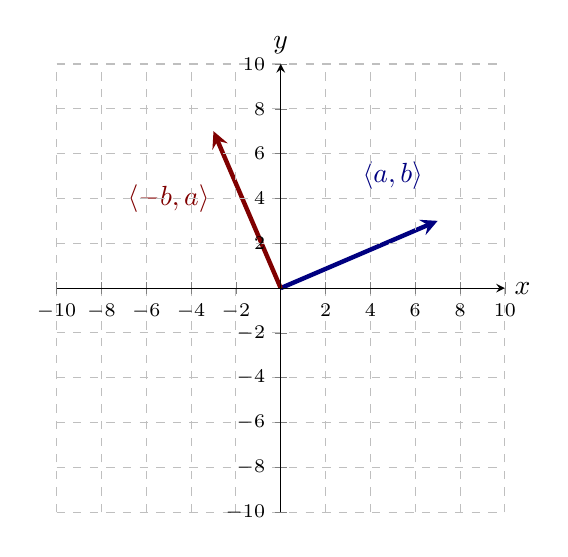
\begin{tikzpicture}
  \begin{axis}[
            domain=-10:10, ymax=10, xmax=10, ymin=-10, xmin=-10,
            axis lines =center, xlabel=$x$, ylabel=$y$, grid = major, grid style={dashed},
            unit vector ratio*=1 1 1,
            ytick={-10,-8,-6,-4,-2,2,4,6,8,10},
            xtick={-10,-8,-6,-4,-2,2,4,6,8,10},
            yticklabels={$-10$,$-8$,$-6$,$-4$,$-2$,$2$,$4$,$6$,$8$,$10$}, 
            xticklabels={$-10$,$-8$,$-6$,$-4$,$-2$,$2$,$4$,$6$,$8$,$10$},
            ticklabel style={font=\scriptsize},
            every axis y label/.style={at=(current axis.above origin),anchor=south},
            every axis x label/.style={at=(current axis.right of origin),anchor=west},
            axis on top
          ]


            \draw[penColor,ultra thick,->] (axis cs:0,0) -- (axis cs:7,3);
            \draw[penColor2,ultra thick,->] (axis cs:0,0) -- (axis cs:-3,7);

            \node at (axis cs:5,5) [penColor] {$\langle a, b \rangle$};
            \node at (axis cs:-5,4) [penColor2] {$\langle -b, a \rangle$};




  \end{axis}
\end{tikzpicture}
\end{image}





\begin{center}
\textbf{\textcolor{red!80!black}{Multiplication by $\langle 0, 1 \rangle$ turns $\langle a, b \rangle$ into $\langle -b, a \rangle$.}}
\end{center}




What else should multiplication do? \\


Addition and multiplication of vectors should behave like addition and multiplication of real numbers.  Namely, the \textbf{\textcolor{purple!85!blue}{distributive property}} should hold.

And, we have scalar multiplication.

And, we have $90^{\circ}$ turning.

Puting all of this together, we get something like this:



\begin{align*}
\langle a, b \rangle  * \langle c, d \rangle & = \langle a, b \rangle  * (  c \cdot \langle 1, 0 \rangle    +  d \cdot \langle 0, 1 \rangle    )    \\
    & = \langle a, b \rangle \cdot c \cdot \langle 1, 0 \rangle     +      \langle a, b \rangle \cdot d \cdot \langle 0, 1 \rangle      \\
    & = c \cdot \langle a, b \rangle *  \langle 1, 0 \rangle     +    d \cdot  \langle a, b \rangle *  \langle 0, 1 \rangle      \\
    & = c \cdot \langle a, b \rangle   + d \cdot  \langle -b, a \rangle \\
    & =  \langle c a, c b \rangle   +   \langle -b d, a d \rangle \\
    & =  \langle c a - b d, c b + a d \rangle   
\end{align*} 







\begin{definition}  \textbf{\textcolor{green!50!black}{Vector Multiplication}}  


\[    \langle a, b \rangle  * \langle c, d \rangle =   \langle c a - b d, c b + a d \rangle   \]


\end{definition}








\begin{example} Vector Multiplication

Compute  $\langle 3, -1 \rangle  * \langle 2, 4 \rangle$

\begin{explanation}


\[
\langle 3, -1 \rangle  * \langle 2, 4 \rangle = \langle 2 \cdot 3 - (-1) \cdot 4, 2 \cdot (-1) + 3 \cdot 4 \rangle = \langle 10, 10 \rangle 
\]
\end{explanation}

\end{example}











\begin{example} Real Number Multiplication

Compute  $3 \cdot 2 = \langle 3, 0 \rangle  * \langle 2, 0 \rangle$

\begin{explanation}


\[
\langle 3, 0 \rangle  * \langle 2, 0 \rangle = \langle 2 \cdot 3 - 0 \cdot 0, 2 \cdot 0 + 3 \cdot 0 \rangle = \langle 6, 0 \rangle 
\]
\end{explanation}

\end{example}




\begin{question} 


Compute  $\langle 1, 2 \rangle  * \langle -2, 3 \rangle = \left\langle \answer{-8}, \answer{-1} \right\rangle $



\end{question}











\begin{center}
\textbf{\textcolor{green!50!black}{ooooo-=-=-=-ooOoo-=-=-=-ooooo}} \\

more examples can be found by following this link\\ \link[More Examples of Representing Numbers]{https://ximera.osu.edu/csccmathematics/precalculus2/precalculus2/representingNumbers/examples/exampleList}

\end{center}





\end{document}
